% ZHOU-SOURCE-PAGE: 121 PRINTED: 105

\section{Stochastic Process and Stochastic Calculus}

In this chapter, we cover a few topics---Markov chain, random walk and martingale,
dynamic programming---that are often not included in introductory probability courses.
Unlike basic probability theory, these tools may not be considered to be standard
requirements for quantitative researchers/analysts. But a good understanding of these
topics can simplify your answers to many interview problems and give you an edge in
the interview process. Besides, once you learn the basics, you'll find many interview
problems turning into fun-to-solve math puzzles.

\subsection{Markov Chain}

A Markov chain is a sequence of random variables $X_0,X_1,\cdots,X_n,\cdots$ with the
Markov property that given the present state, the future states and the past states are
independent:

\[
P\{X_{n+1}=j\mid X_n=i,X_{n-1}=i_{n-1},\cdots,X_0=i_0\}
=p_{ij}=P\{X_{n+1}=j\mid X_n=i\}
\]

for all $n$, $i_0,\cdots,i_{n-1}$, $i$ and $j$, where $i,j\in\{1,2,\cdots,M\}$
represent the state space $S=\{s_1,s_2,\cdots,s_M\}$ of $X$.

In other words, once the current state is known, past history has no bearing on the
future. For a homogeneous Markov chain, the transition probability from state $i$ to
state $j$ does not depend on $n$.\footnote[1]{In this chapter, we only consider finite-state homogeneous Markov chains (i.e., transition probabilities do not change over time).} A Markov chain with $M$ states can be completely described by an
$M\times M$ transition matrix $P$ and the initial probabilities $P(X_0)$.

\noindent\textbf{Transition matrix:}
$P=\{p_{ij}\}=\left[\begin{array}{cccc}
p_{11}&p_{12}&\cdots&p_{1M}\\
p_{21}&p_{22}&\cdots&p_{2M}\\
\vdots&\vdots&\ddots&\vdots\\
p_{M1}&p_{M2}&\cdots&p_{MM}
\end{array}\right]$,
where $p_{ij}$ is the transition probability from state $i$ to state $j$.

\noindent\textbf{Initial probabilities:}
$P(X_0)=(P(X_0=1),P(X_0=2),\cdots,P(X_0=M))$,
$\displaystyle\sum_{i=1}^{M}P(X_0=i)=1$.

\noindent\textbf{The probability of a path:}
$P(X_1=i_1,X_2=i_2,\cdots,X_n=i_n\mid X_0=i_0)
=p_{i_0i_1}p_{i_1i_2}\cdots p_{i_{n-1}i_n}$

\noindent\textbf{Transition graph:} A transition graph is often used to express the
transition matrix graphically. The transition graph is more intuitive than the matrix,
and it emphasizes

% ZHOU-SOURCE-PAGE: 122 PRINTED: 106

possible and impossible transitions. Figure~\ref{fig:zhou-figure-5-1} shows the transition
graph and the transition matrix of a Markov chain with four states:

\begin{figure}[ht]
\centering
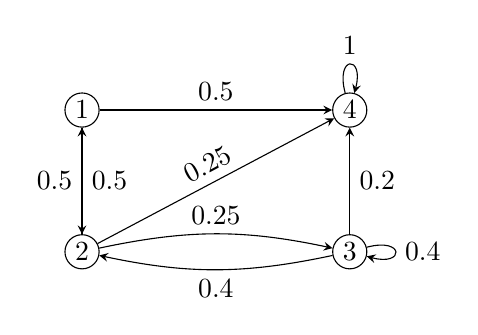
\begin{tikzpicture}[>=stealth, node distance=1.6cm]
  \node[draw,circle,inner sep=1.5pt] (one) at (0,1.8) {$1$};
  \node[draw,circle,inner sep=1.5pt] (two) at (0,0) {$2$};
  \node[draw,circle,inner sep=1.5pt] (three) at (3.4,0) {$3$};
  \node[draw,circle,inner sep=1.5pt] (four) at (3.4,1.8) {$4$};
  \draw[->] (one) -- node[above] {$0.5$} (four);
  \draw[->] (one) -- node[left] {$0.5$} (two);
  \draw[->] (two) -- node[right] {$0.5$} (one);
  \draw[->] (two) to[bend left=12] node[above] {$0.25$} (three);
  \draw[->] (three) to[bend left=12] node[below] {$0.4$} (two);
  \draw[->] (three) -- node[right] {$0.2$} (four);
  \draw[->] (two) -- node[sloped,above] {$0.25$} (four);
  \draw[->] (four) to[loop above] node {$1$} (four);
  \draw[->] (three) to[loop right] node {$0.4$} (three);
\end{tikzpicture}
\qquad
\begin{tikzpicture}[baseline=(current bounding box.center)]
  \node (mat) {$
    P=\{p_{ij}\}=\left[\begin{array}{cccc}
    0&0.5&0&0.5\\
    0.5&0&0.25&0.25\\
    0&0.4&0.4&0.2\\
    0&0&1&0
    \end{array}\right]
  $};
  \node[above=1pt of mat.north] {$i=1\quad 2\quad 3\quad 4$};
  \node[right=3pt of mat.east] {$\begin{array}{c}j\\1\\2\\3\\4\end{array}$};
\end{tikzpicture}
\caption{Transition graph and transition matrix of the Play}
\label{fig:zhou-figure-5-1}
\end{figure}

\noindent\textbf{Classification of states}

State $j$ is accessible from state $i$ if there is a directed path in the transition graph
from $i$ to $j$ ($\exists n$ such that $p^{(n)}_{ij}>0$). Let
$T_{ij}=\min(n:X_n=j\mid X_0=i)$, then $P(T_{ij}<\infty)>0$ if and only if state $j$
is accessible from state $i$. States $i$ and $j$ communicate if $i$ is accessible from $j$
and $j$ is accessible from $i$. In Figure~\ref{fig:zhou-figure-5-1}, state 3 and 1 communicate.
State 4 is accessible form state 1, but they do not communicate since state 1 is not
accessible from state 4.

We say that state $i$ is recurrent if for every state $j$ that is accessible from $i$, $i$
is also accessible from $j$ ($\forall j$, $P(T_{ij}<\infty)>0\Rightarrow
P(T_{ji}<\infty)=1$). A state is called \textbf{transient} if it is not recurrent
($\exists j$, $P(T_{ij}<\infty)>0$ and $P(T_{ji}<\infty)<1$). In Figure~\ref{fig:zhou-figure-5-1},
only state 4 is recurrent. States 1, 2 and 3 are all transient since 4 is accessible from
1/2/3, but 1/2/3 are not accessible from 4.

\noindent\textbf{Absorbing Markov chains:} A state $i$ is called absorbing if it is
impossible to leave this state ($p_{ii}=1$, $p_{ij}=0$, $\forall j\ne i$). A Markov chain
is absorbing if it has at least one absorbing state and if from every state it is possible
to go to an absorbing state. In Figure~\ref{fig:zhou-figure-5-1}, state 4 is an absorbing
state. The corresponding Markov chain is an absorbing Markov chain.

\noindent\textbf{Equations for absorption probability:} The probability to reach a
specific absorbing state $s$, $a_1,\cdots,a_M$, are unique solutions to equations
$a_s=1$, $a_i=0$ for all absorbing state(s) $i\ne s$, and
$a_i=\displaystyle\sum_{j=1}^{M}a_jp_{ij}$ for all transient states $i$. These equations
can be easily

% ZHOU-SOURCE-PAGE: 123 PRINTED: 107

derived using the law of total probability by conditioning the absorption probabilities on
the next state.

\noindent\textbf{Equations for the expected time to absorption:} The expected times to
absorption, $\mu_1,\cdots,\mu_M$, are unique solutions to the equations $\mu_i=0$ for
all absorbing state(s) $i$ and $\mu_i=1+\displaystyle\sum_{j=1}^{M}p_{ij}\mu_j$ for
all transient states $i$. These equations can be easily derived using the law of total
expectation by conditioning the expected times to absorption on the next state. The number
1 is added since it takes one step to reach the next state.

\problem{Gambler's ruin problem}
Player $M$ has \$1 and player $N$ has \$2. Each game gives the winner \$1 from the other.
As a better player, $M$ wins 2/3 of the games. They play until one of them is bankrupt.
What is the probability that $M$ wins?

\solution
The most difficult part of Markov chain problems often lies in how to choose the right
state space and define the transition probabilities $p_{ij}$'s, $\forall i,j$. This problem
has fairly straightforward states. You can define the state space as the combination of
the money that player $M$ has ($m$) and the money that player $N$ has ($n$):
$\{(m,n)\}=\{(3,0),(2,1),(1,2),(0,3)\}$. (Neither $m$ nor $n$ can be negative since
the whole game stops when one of them goes bankrupt.) Since the sum of the dollars of both
players is always \$3, we can actually simplify the state space using only $m$:
$\{m\}=\{0,1,2,3\}$.

The transition graph and the corresponding transition matrix are shown in
Figure~\ref{fig:zhou-figure-5-2}.

\begin{figure}[ht]
\centering
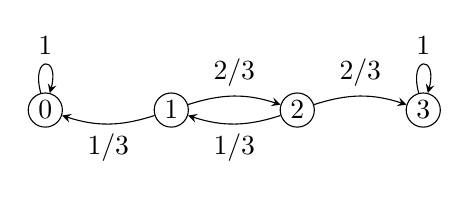
\begin{tikzpicture}[>=stealth]
  \node[draw,circle,inner sep=1.5pt] (zero) at (0,0) {$0$};
  \node[draw,circle,inner sep=1.5pt] (one) at (1.6,0) {$1$};
  \node[draw,circle,inner sep=1.5pt] (two) at (3.2,0) {$2$};
  \node[draw,circle,inner sep=1.5pt] (three) at (4.8,0) {$3$};
  \draw[->] (zero) to[loop above] node {$1$} (zero);
  \draw[->] (one) to[bend left=18] node[above] {$2/3$} (two);
  \draw[->] (two) to[bend left=18] node[above] {$2/3$} (three);
  \draw[->] (one) to[bend left=18] node[below] {$1/3$} (zero);
  \draw[->] (two) to[bend left=18] node[below] {$1/3$} (one);
  \draw[->] (three) to[loop above] node {$1$} (three);
\end{tikzpicture}
\qquad
\begin{tikzpicture}[baseline=(current bounding box.center)]
  \node (mat) {$
    P=\{p_{ij}\}=\left[\begin{array}{cccc}
    p_{0,0}&p_{0,1}&p_{0,2}&p_{0,3}\\
    p_{1,0}&p_{1,1}&p_{1,2}&p_{1,3}\\
    p_{2,0}&p_{2,1}&p_{2,2}&p_{2,3}\\
    p_{3,0}&p_{3,1}&p_{3,2}&p_{3,3}
    \end{array}\right]
    =\left[\begin{array}{cccc}
    1&0&0&0\\
    1/3&0&2/3&0\\
    0&1/3&0&2/3\\
    0&0&0&1
    \end{array}\right]
  $};
  \node[above=1pt of mat.north] {$i=0\qquad 1\qquad 2\qquad 3$};
  \node[left=3pt of mat.west] {$\begin{array}{c}j\\0\\1\\2\\3\end{array}$};
\end{tikzpicture}
\caption{Transition matrix and transition graph for Gambler's ruin problem}
\label{fig:zhou-figure-5-2}
\end{figure}

The initial state is $X_0=1$ ($M$ has \$1 at the beginning). At state 1, the next state is
0 ($M$ loses a game) with probability 1/3 and 2 ($M$ wins a game) with probability 2/3.
So $p_{1,0}=1/3$ and $p_{1,2}=2/3$. Similarly we can get $p_{2,1}=1/3$ and
$p_{2,3}=2/3$. Both state 3 ($M$ wins the whole game) and state 0 ($M$ loses the whole
game) are absorbing states.

To calculate the probability that $M$ reaches absorbing state 3, we can apply absorption
probability equations:

% ZHOU-SOURCE-PAGE: 124 PRINTED: 108

$a_3=1$, $a_0=0$, and
$a_1=\displaystyle\sum_{j=0}^{3}p_{1,j}a_j$, $a_2=\displaystyle\sum_{j=0}^{3}p_{2,j}a_j$.

Plugging in the transition probabilities using either the transition graph or transition
matrix, we have

\[
\begin{aligned}
a_1&=1/3\times0+2/3\times a_2\\
a_2&=1/3\times a_1+2/3\times1
\end{aligned}
\quad\Longrightarrow\quad
\begin{cases}
a_1=4/7,\\
a_2=6/7.
\end{cases}
\]

So, starting from \$1, player $M$ has $4/7$ probability of winning.

\problem{Dice question}
Two players bet on roll(s) of the total of two standard six-face dice. Player $A$ bets
that a sum of 12 will occur first. Player $B$ bets that two consecutive 7s will occur first.
The players keep rolling the dice and record the sums until one player wins. What is the
probability that $A$ will win?

\solution
Many of the simple Markov chain problems can be solved using pure conditional probability
argument. It is not surprising considering that Markov chain is defined as conditional
probability:

\[
P\{X_{n+1}=j\mid X_n=i,X_{n-1}=i_{n-1},\cdots,X_0=i_0\}
=p_{ij}=P\{X_{n+1}=j\mid X_n=i\}.
\]

So let's first solve the problem using conditional probability arguments. Let $P(A)$ be
the probability that $A$ wins. Conditioning $P(A)$ on the first throw's sum $F$, which has
three possible outcomes $F=12$, $F=7$ and $F\notin\{7,12\}$, we have

\[
\begin{aligned}
P(A)&=P(A\mid F=12)P(F=12)+P(A\mid F=7)P(F=7)\\
&\quad+P(A\mid F\notin\{7,12\})P(F\notin\{7,12\}).
\end{aligned}
\]

Then we tackle each component on the right hand side. Using simple permutation, we can
easily see that $P(F=12)=1/36$, $P(F=7)=6/36$, $P(F\notin\{7,12\})=29/36$. Also it
is obvious that $P(A\mid F=12)=1$ and $P(A\mid F\notin\{7,12\})=P(A)$. (The game
essentially starts over again.) To calculate $P(A\mid F=7)$, we need to further condition
on the second throw's total, which again has three possible outcomes: $E=12$, $E=7$, and
$E\notin\{7,12\}$.

\[
\begin{aligned}
P(A\mid F=7)
&=P(A\mid F=7,E=12)P(E=12\mid F=7)\\
&\quad+P(A\mid F=7,E=7)P(E=7\mid F=7)\\
&\quad+P(A\mid F=7,E\notin\{7,12\})\\
&\qquad{}\times P(E\notin\{7,12\}\mid F=7)\\
&=P(A\mid F=7,E=12)\times1/36
 +P(A\mid F=7,E=7)\times6/36\\
&\quad+P(A\mid F=7,E\notin\{7,12\})\times29/36\\
&=1\times1/36+0\times6/36+P(A)\times29/36\\
&=1/36+29/36P(A).
\end{aligned}
\]

Here the second equation relies on the independence between the second and the first
rolls. If $F=7$ and $E=12$, $A$ wins; if $F=7$ and $E=7$, $A$ loses; if $F=7$ and

% ZHOU-SOURCE-PAGE: 125 PRINTED: 109

$E\notin\{7,12\}$, the game essentially starts over again. Now we have all the necessary
information for $P(A)$. Plugging it into the original equation, we have

\[
\begin{aligned}
P(A)&=P(A\mid F=12)P(F=12)+P(A\mid F=7)P(F=7)\\
&\quad+P(A\mid F\notin\{7,12\})P(F\notin\{7,12\})\\
&=1\times1/36+6/36\times(1/36+29/36P(A))\\
&\quad+29/36P(A)
\end{aligned}
\]

Solving the equation, we get $P(A)=7/13$.

This approach, although logically solid, is not intuitively appealing. Now let's try a
Markov approach. Again the key part is to choose the right state space and define the
transition probabilities. It is apparent that we have two absorbing states, 12 ($A$ wins)
and 7-7 ($B$ wins), at least two transient states, $S$ (starting state) and 7 (one 7
occurs, yet no 12 or 7-7 occurred). Do we need any other states? Theoretically, you can
have other states. In fact, you can use all combination of the outcomes of one roll and two
consecutive rolls as states to construct a transition matrix and you will get the same final
result. Nevertheless, we want to consolidate as many equivalent states as possible. As we
just discussed in the conditional probability approach, if no 12 has occurred and the most
recent roll did not yield 7, we essentially go back to the initial starting state $S$. So all
we need are states $S$, 7, 7-7 and 12. The transition graph and probability to reach state
12 are shown in Figure~\ref{fig:zhou-figure-5-3}.

\begin{figure}[ht]
\centering
\begin{tikzpicture}[>=stealth]
  \node[draw,circle,inner sep=1.5pt] (s) at (0,0) {$S$};
  \node[draw,circle,inner sep=1.5pt] (seven) at (1.8,0) {$7$};
  \node[draw,ellipse,inner sep=3pt] (sevenseven) at (3.8,0.9) {$7$-$7$};
  \node[draw,ellipse,inner sep=3pt] (twelve) at (3.8,-1.1) {$12$};
  \draw[->] (s) to[loop left] node {$29/36$} (s);
  \draw[->] (s) to[bend left=12] node[above] {$6/36$} (seven);
  \draw[->] (seven) to[bend left=14] node[above] {$6/36$} (sevenseven);
  \draw[->] (seven) to[bend left=14] node[below] {$29/36$} (s);
  \draw[->] (seven) to[bend right=12] node[below] {$1/36$} (twelve);
  \draw[->] (sevenseven) to[loop above] node {$1$} (sevenseven);
  \draw[->] (twelve) to[loop below] node {$1$} (twelve);
\end{tikzpicture}
\qquad
\begin{minipage}[c]{0.42\linewidth}
\centering
\textbf{Probability to absorption state 12}
\[
\begin{gathered}
\begin{aligned}
a_{12}&=1,\quad a_{7-7}=0,\\
a_S&=1/36\times1+6/36\times a_7\\
&\quad+29/36\times a_S,\\
a_7&=1/36\times1+6/36\times0\\
&\quad+29/36\times a_S
\end{aligned}\\
\quad\Longrightarrow\quad a_S=7/13
\end{gathered}
\]
\end{minipage}
\caption{Transition graph and probability to absorption for dice rolls}
\label{fig:zhou-figure-5-3}
\end{figure}

Here the transition probability is again derived from conditional probability arguments.
Yet the transition graph makes the process crystal clear.

\subsubsection{Coin triplets}

\noindent\textbf{Part A.} If you keep on tossing a fair coin, what is the expected number
of tosses such that you can have $HHH$ (heads heads heads) in a row? What is the expected
number of tosses to have $THH$ (tails heads heads) in a row?

\solution
The most difficult part of Markov chain is, again, to choose the right state space. For
the $HHH$ sequence, the state space is straightforward. We only need four states: $S$ (for
the starting state when no coin is tossed or whenever a $T$ turns up before $HHH$), $H$,
$HH$, and $HHH$. The transition graph is
